\chapter{Onde nei plasmi e smorzamento di Landau}

\epigraph{
	Riferimenti: cap. 9-10-11 di \emph{Fisica dei plasmi} di Pucella-Segre
}{}

Ricordiamo dei risultati già ottenuti per poi sviluppare una descrizione delle onde di plasma aggiornata alle nuove descrizioni che abbiamo sviluppato negli ultimi capitoli (teoria cinetica e magnetoidrodinamica).

\subsection{Onde acustiche}

Abbiamo già visto nel capitolo 2 come, partendo dalle equazioni fluide linearizzate abbiamo visto come una perturbazione di pressione o densità genera un'onda di pressione che si propaga con velocità $c_s$ ($\sqrt{\gamma P_0 /\rho_0}$):

\[ \begin{cases}
	\displaystyle\frac{\partial }{\partial t} (\delta \rho)\ =\ \rho_0\, \displaystyle\frac{\partial}{\partial x} (\delta u)\qquad \quad\text{eq. di continuità linearizzata}\ ,\\ \\
	\displaystyle\frac{\partial }{\partial t} (\delta u)\ =\ - \displaystyle\frac{1}{\rho_0}\,\frac{\partial}{\partial x} (\delta P)\qquad \text{eq. del moto linearizzata}\ ,\\ \\
	\delta P\, =\, c_s^2\, \delta \rho\qquad \qquad\qquad \text{eq. politropica linearizzata}\ .
\end{cases} 
\quad \implies \quad 
\frac{\partial^2}{\partial t^2} (\delta \rho)\ =\ c_s^2\ \frac{\partial^2}{\partial x^2} (\delta \rho)\]

Assumendo come soluzioni delle onde piane per pressioni e velocità ($\delta \rho (x, t) = \hat \rho e^{i(kx-\omega t)}$ e $\delta u (x, t) = \hat u e^{i(kx-\omega t)}$) e facendo una trasformata di Fourier ($\partial_x\rightarrow ik$, $\partial_t\rightarrow -i\omega$) si è trovata la relazione di dispersione:
\begin{equation}
	\label{acoustic wave}
	\omega^2\ =\ k^2\, c_s^2
\end{equation}


%
%
%
\subsection{Onde di plasma}
Sempre nel capitolo 2 partendo dalle equazioni fluide in trasformata di Fourier, questa volta considerando il termine di forza dovuta al campo, ci siamo chiesti come si propagasse una fluttuazione non di sola pressione, considerando gli ioni come fissi perché si presuppone che gli elettroni rispondano alle fluttuazioni del campo su scale di tempo ben più corte. 

Abbiamo aggiunto anche l'equazione di Poisson unita a $\vec E=\vec \nabla \phi$:

\[\begin{cases}
	-\, i\omega\,\delta n_e\ +\ i k\, n_{0, e}\,\delta u_e\ =\ 0\ , \\
	-\, i\omega\, m_e\, n_{0, e}\, \delta u\ =\ ik\, e n_{0, e}\, \delta \phi\, -\, ik\,\delta P\ , \\
	-\,k^2\, \delta \phi\ =\ 4\pi e\, \delta n_e\ .
\end{cases}\]

Da qui avevamo notato la presenza di 4 incognite per sole 3 equazioni, abbiamo risolto il problema in due modi:
\begin{itemize}
	\item Chiusura plasma freddo: non consideriamo il termine di pressione ($\delta P\sim 0$) e troviamo così una relazione di dispersione che definisce la frequenza di plasma elettronica 
	\begin{equation}
		\label{onde di plasma freddo}
		\omega^2\ =\ \frac{4\pi\, e^2\, n_{0, e}}{m_e} \ \equiv\  \omega^2_{p,e}\ \ ;
	\end{equation}
	\item Chiusura politropica: andiamo ad usare come per le onde acustiche l'ipotesi che il plasma segua una politropica, da cui $\delta P=\gamma T_{0,e}\delta n_e $, così che si trovi la relazione di dispersione
	\[\omega^2=\omega^2_p+\gamma k^2v_{th,e}\ \ .\]
\end{itemize}

%
%
\subsubsection{Onda elettromagnetica che investe un plasma}

\epigraph{
	Riferimenti: cap. 5 del Krall, sezione "\emph{cold-plasma, unmagnetised, linear response}"
}{}

Come ultimo tipo di onde già descritto nel capitolo 2, ci siamo chiesti come reagisse il plasma ad un'onda elettromagnetica che lo investe, per farlo abbiamo usato l'equazione del moto fluida con termine di forza elettrica non considerando il campo magnetico (plasma non magnetizzato, $\vec B=0$) e considerando il plasma freddo ($\vec \nabla P\sim 0$). 

A questa equazione abbiamo unito le equazioni di Maxwell:

\[\begin{cases}
	n_\alpha \frac{\partial \delta u_\alpha}{\partial t}\ =\ \frac{n_\alpha}{m_\alpha}\, q_\alpha\, \vec E\ ,\\
	\vec \nabla \times \vec B \ =\ \frac{1}{c}\frac{\partial \vec E}{\partial t} + \frac{4\pi}{c}\vec j\ ,\\
	\vec \nabla \times \vec E = \frac{1}{c}\frac{\partial \vec B}{\partial t}\ .
\end{cases}\]

Anche qui si fa una trasformata di Fourier e si usa la prima equazione per trovare un'espressione di $\delta \vec u_\alpha$ da usare nella corrente $\vec j = \sum_\alpha q_\alpha n_{0,\alpha}\delta \vec u_\alpha$, così che:

\[\begin{cases}
	\vec j\ =\ -\frac{i}{\omega}\,  \sum_\alpha \frac{q^2_\alpha n_{0,\alpha} }{m_\alpha}\,\vec E\ ,\\
	i\vec k \times \vec B \ =\ -\frac{i\omega}{c}\,\vec E\, +\, \frac{4\pi}{c}\,\vec j\ ,\\
	\vec B\ =\ \frac{c}{\omega}\vec k\times \vec E\ .
\end{cases}\]

Per risolvere il sistema si inseriscono le espressioni di $\vec B,\, \vec j$ della prima e terza equazione nella seconda equazione e si usa la definizione di frequenza di plasma $\omega_P^2=\omega^2_{P,e}+\omega^2_{P,i}\sim\omega^2_{P,e}$ (dove $\omega_P,e$ era stata già definita come frequenza di plasma elettronica $\equiv \sqrt{4\pi n_{0,\alpha} q^2_\alpha / m_\alpha}$ )

Da qui abbiamo osservato la possibilità di dividere il risultato per la propagazione nel caso $\vec k\perp \vec E$ e quella nel caso $\vec k\parallel \vec E$, questo perché k è in una direzione e il campo può essere scomposto in una componente parallela ed una trasversa, con l'aiuto della relazione $-(\vec k\cdot \vec E)\vec k+k^2\vec E = \frac{\omega^2}{c^2} \left(1-\frac{\omega^2_P}{\omega^2}\right)\vec E$ abbiamo trovato:
\begin{itemize}
	\item Per il caso di onda elettromagnetica trasversa, $\vec k\perp \vec E$, si ha la relazione di dispersione
	\[\omega^2\ =\ \omega_P^2\, +\, k^2\,c^2\ \ ;\]
	\item Per il caso di onda elettromagnetica con propagazione parallela al campo, $\vec k\parallel \vec E$, si ha relazione di dispersione simile al caso di onde di plasma freddo
	\[\omega^2\ =\ \omega^2_P\]
\end{itemize}


\section{Onde ion-acustic}


Onde elettrostatiche di tipo acustico/sonoro, si possono ricavare da vlasov ma noi non lo facciamo, le ricaviamo con il modello a due fluidi. 

Se partissimo direttamente dall'MHD non troveremmo le onde di plasma (e il landau damping), ma noi invece le troveremo (questa parte è un po' poco chiara, si fa facilmente confusione fra tutti questi tipi di onde in diversi regimi, ma vediamo come rimettere il tutto in ordine).

Abbiamo un plasma non magnetizzato:

\[\vec E_0=0 \implies \vec E=\vec E_1\ ;\qquad
\vec B_0=0\implies \vec B=\vec b\ ; \qquad
\vec u_0=0\implies \vec u=\vec u_1\] 

il termine $\vec u_1\times\vec b$ è del second'ordine ed è pertanto per noi nullo, significa che la nostra onda è polarizzata longitudinalmente e non abbiamo onde elettromagnetiche che avrebbero bisogno del campo magnetico,

\[\vec E\parallel\vec u\parallel\vec k\]

La velocità di fase dell'onda ion-acustic è molto minore delle velocità termiche elettroniche in gioco: 

\[v_{th,I}\ll v_f \ll v_{th,e} \] 

i tempi scale sono tali da avere una risposta inerziale (adiabatica) da parte degli ioni e una risposta termica (isoterma) da parte degli elettroni. questo implica che devo usare due politropiche diverse per le due specie.   

\paragraph{Equazioni di base: } 
\[n_\alpha=n_{0\alpha}+n_{1\alpha}\hspace{1cm}P_\alpha=P_{0\alpha}+P_{1\alpha}\hspace{1cm}\alpha=I,e\]

\[\begin{aligned}
	\text{equazione di continuità linearizzata}\qquad \qquad  
	& \partial_tn_{1\alpha }+\nabla\cdot(n_{0\alpha}\vec u_{1\alpha})=0\\ 
	\text{equazione del moto linearizzata} \qquad \qquad
	& m_\alpha\, n_{0\alpha}\,\partial_t\vec u_{1\alpha}\ =\ -\nabla P_{1\alpha}\,+\,n_{0\alpha}q_{\alpha}\,(\vec E+\cancelto{0}{\frac{\vec u_{1\alpha}\times\vec b}{c}})\\
	\text{chiusura politropica linearizzata} \qquad \qquad
	& P_{1\alpha}\ =\ \gamma_\alpha\frac{P_{0\alpha}}{n_{0\alpha}}n_{1\alpha}\ \underset{\begin{cases} P=nT\\ v_{th}^2=T/m \end{cases}}{=}\ \gamma_\alpha\,  v^2_{th}\, m_\alpha\,n_{1\alpha}
\end{aligned}\]


\paragraph{soluzione onda piana e relazione di dispersione: } 
Cerco una soluzione ad onda piana $\sim e^{i(\vec k\cdot\vec r-\omega t)}$, trovo un sistema di equazioni che se risolte mi danno la relazione di dispersione.  

Risulta utile definire una sorta di "\underline{velocità del suono per la specifica specie}"

\[\boxed{ v^2_{0\alpha}=\frac{\gamma_\alpha P_{0\alpha}}{m_\alpha n_{0\alpha}} }\] 

Facciamo una trasformata di Fourier e togliamo i segni di vettore perché il nostro problema adesso è unidimensionale:

\[\begin{cases}
	-i\omega\,n_{1\alpha}\,+\,ik\,n_{0\alpha}u_\alpha\ =\ 0
	\\
	i\,\omega m\,_\alpha n_{0\,\alpha}\,u_\alpha\ =\ -iP_{1\alpha}k\,+\, n_{0\alpha}q_{\alpha}\, E
	\\
	P_{1\alpha}\ =\ \gamma_\alpha\, \frac{P_{0\alpha}}{n_{0\alpha}}\, n_{1\alpha}    
\end{cases} \quad \implies \quad u_\alpha\ =\ \frac{iq_\alpha}{m_\alpha}\,\frac{\omega}{\omega^2-k^2v_{0\alpha}^2}\, E\] 

Adesso che abbiamo le velocità possiamo ricavare la corrente totale moltiplicando ogni equazione per $n_\alpha q_\alpha$ e sommando sulle $\alpha$:

\[\begin{aligned}\sigma E\,=\,J\, &=\,\sum_\alpha J_\alpha\,=\,\sum_\alpha n_\alpha q_\alpha u_\alpha\\ 
	&=\, \frac{i\omega}{4\pi} \sum_\alpha \underset{\omega^2_{P,\,\alpha}}{\underbrace{\frac{4\pi n_{0,\alpha}q^2_\alpha}{m_\alpha}}}\, E\, \left(\frac{1}{\omega^2 - k^2 v^2_{0,\alpha}}\right) \\
	&=\, \underset{\sigma}{\underbrace{\frac{i\omega}{4\pi} \sum_\alpha \omega^2_{P,\, \alpha} \left( \frac{ 1 }{ \omega^2-k^2v^2_{0,\alpha} } \right)}}\, E
\end{aligned}\]


Abbiamo quindi un'espressione per la \underline{suscettività elettrica} $\sigma$, mentre per la \underline{permittività} usiamo l'espressione in eq.(\ref{permittività})

\begin{equation}
	\label{permittività}
	\epsilon=1+\frac{4\pi i}{\omega}\sigma
\end{equation}

\[\epsilon\ =\ 1\, - \, \frac{\omega_{pI}^2}{\omega^2-k^2v_{0I}^2}\, -\, \frac{\omega_{pe}^2}{\omega^2-k^2v_{0e}^2}\] 

Se trascuriamo il termine degli ioni, ritroviamo le onde di plasma freddo con correzione termica, come ci aspetteremmo. 


\paragraph{caso $\epsilon=0$: }
Per trovare la relazione generale imponiamo di trovarci in un modo normale isotropo, $\epsilon=0$. 
Dobbiamo ricordare che $\omega_{pI}^2\sim\frac{1}{m_I}\ll\omega_{pe}^2\sim\frac{1}{m_e}$ ed andare a risolvere l'espressione di quarto grado per $\omega^2$:

\[0 \ =\ (\omega^2-k^2v_{0e}^2)\,(\omega^2-k^2v_{0I}^2)\, -\,\omega_{pI}^2\,(\omega^2-k^2v_{0e}^2)\, -\, \omega_{pe}^2\, (\omega^2-k^2v_{0I}^2)\]

\[\omega^4\, -\,\left[k^2(v^2_{0,\,e}+v^2_{0,\,I})+ \omega^2_{p,\,e} + \omega^2_{p,\,I}\right]\omega^2\, +\, [k^4 v^2_{0,\,e} v^2_{0,\,I} + k^2(\omega^2_{p,\,I}v^2_{0,\,e}+\omega^2_{p,\,e}v^2_{0,\,I})]\ =\ 0\]

Per procedere più agevolmente prendiamo $\omega^4-A\omega^2+C=0$ poniamo $\omega^2=\frac{A}{2}[1\pm(1-B)^\frac{1}{2}]$, con un nuovo $B=4C/A^2$. Vediamo che $B$ è piccolo, $B\,\sim\,m_e/\,m_I\,\ll\, 1$, quindi possiamo fare un'approssimazione di Taylor (per intenderci il numeratore va come $\displaystyle\frac{1}{m_Im_e}$ e il denominatore va come $\displaystyle\frac{1}{m_e^2}$.).

%\[\omega^2\ =\ \frac{1}{2}\ \big[k^2(v_{0I}^2+v_{0e}^2)+\omega_{pe}^2 \big]\ \bigg\{ 1\pm \bigg[ 1-\frac{2k^2 v_{0e}^2\omega_{pI}^2+v_{0I}^2\omega_{pe}^2+k^2v_{0I}^2v_{0e}^2}{ \big(k^2(v_{0I}^2+v_{0e}^2)+\omega_{pe}^2   \big)^2}\bigg]^{1/2} \bigg\} \] 

\[\omega^2\ \sim\ \frac{A}{2}\,\left[1\,\pm\,\big(1-\frac{B}{2}\big)\right]
\quad \implies \qquad 
\begin{cases}
	\omega_{th}^2\ \simeq\ A\ \simeq\ k^2v_{0e}^2+\omega_{pe}^2\\
	\omega^2_{IA}\ \simeq\ \frac{AB}{4}\ =\ \frac{C}{A}\ =\ \frac{k^4 v^2_{0,\,e} v^2_{0,\,I} + k^2(\omega^2_{p,\,I}v^2_{0,\,e}+\omega^2_{p,\,e}v^2_{0,\,I})}{k^2(v^2_{0,\,e}+v^2_{0,\,I})+ \omega^2_{p,\,e} + \omega^2_{p,\,I}}
\end{cases}
\]

Otteniamo due soluzioni, una è la soluzione già trovata delle \underline{onde di plasma con correzione termica} $\omega_{th}$, questo perché stiamo considerando il modello a due fluidi in cui le onde di plasma sono previste. 

L'altra soluzione, $\omega^2_{IA}$, invece è quella che ci interessa.

Si mette ora in evidenza $v_{0e}^2$ a numeratore e denominatore e si riconosce la lunghezza di Debye, $\lambda_{D,\, \alpha}\,=\,v_{th,\,\alpha}/\omega_{P,\,\alpha}$ :  

\[\lambda _{D\alpha}^2\,=\,\frac{v_{th.\alpha}^2}{\omega_{p\alpha}^2}\,\sim\, \frac{v_{0,\alpha}^2}{\omega_{p\alpha}^2},
\qquad\qquad
v_{0I}^2=\frac{\gamma_IP_{0I}}{m_In_{0I}}=\frac{\gamma_IT_{I}}{m_I}
\qquad\qquad
\frac{\lambda^2_{De}}{\lambda^2_{DI}}=\frac{T_e}{T_I}\] 

Otteniamo infine la \underline{relazione di dispersione delle onde Ion-Acoustic}: 
\[\boxed{\frac{\omega^2_\text{IA}}{k^2}\ =\ v_{0I}^2\ \frac{k^2\,+\,\frac{1}{\lambda_\text{De}^2}\,+\,\frac{1}{\lambda_\text{DI}^2}}{k^2\,+\,\frac{1}{\lambda_\text{De}^2}}}\ .\]

\subsubsection{Regimi } Riconosciamo 3 regimi a seconda dell'ordinamento della lunghezza d'onda, andiamo quindi a vedere come $k$ si confronta alle inverse delle lunghezze di Debye inverse. 

\begin{enumerate}
	\item il \underline{caso classico} è quello per cui $k^2\,\ll\, \lambda_{\text{D, e}}^{-2},\,\, \lambda_{\text{D, I}}^{-2}$ :
	
	\[k^2\ll\frac{1}{\lambda_{\text{D, e}}^2}\iff\lambda^2\gg\lambda_{\text{D, e}}^2,\qquad\qquad k^2\ll\frac{1}{\lambda_{\text{D, I}}^2}\iff\lambda^2\gg\lambda_{\text{D, I}}^2\] 
	
	Questa relazione non ci dice in che maniera sono ordinate le $\lambda_D$ e di conseguenza le $T$. in linea di principio è possibile che siano qualsiasi.  
	
	\item  Oscillazioni di plasma degli ioni:
	
	\[k^2\gg\frac{1}{\lambda_{D,e}^2}\iff\lambda^2\ll\lambda_{D,e}^2\ \ ,
	\qquad \quad k^2\ll\frac{1}{\lambda_{DI}^2}\iff\lambda^2\gg\lambda_{DI}^2\] 
	
	Data la prima disuguaglianza, il $k^2$ della relazione di dispersione può essere non considerato al denominatore, ma vista la seconda disuguaglianza anche quello al numeratore può essere ignorato:
	
	\[\lambda_{De}^2\ll\lambda^2\ll\lambda_{DI}^2
	\ \ \implies \ \ 
	T_I\gg T_e\]   
	
	\[\frac{\omega^2}{k^2}\ =\ v_{0I}^2\,\left(1+\frac{\lambda_{De}^2}{\lambda_{DI}^2}\right)\ =\ \frac{\gamma_I}{m_I}\, T_I\, \left(\frac{T_e+T_I}{T_I}\right)\]
	
	\[\boxed{\frac{\omega^2}{k^2}\ =\ \frac{\gamma_I}{m_I}\, (T_e+T_I)}\] 
	
	Questa può essere vista come una sorta di velocità del suono, infatti queste sono le tipiche onde "ion-acustic". Si vede che l'inerzia è data dagli ioni nel senso che compare $m_I$ mentre la risposta termica è data da entrambi, anche se quando $T_I\sim T_e$ tipicamente avviene il Damping di Landau e l'onda non si propaga (a meno che non si faccia una forzatura). 
	Le onde che sopravvivono sono quelle con $T_e\gg T_i$.
	
	\item \[k^2\gg\frac{1}{\lambda_{De}^2}\iff\lambda^2\ll\lambda_{De}^2,\quad k^2\gg\frac{1}{\lambda_{DI}^2}\iff\lambda^2\ll\lambda_{DI}^2\]  Questo caso è praticamente insensato perchè siamo al di sotto delle lunghezze di Debye e praticamente non possiamo nemmeno dire di avere a che fare con un plasma. In questo caso la soluzione ha come relazione di dispersione una relazione analoga alle onde di plasma, ma per gli ioni. 
	\[\omega^2\ =\ \omega_{pI}^2\ +\ k^2\,v_{0I}^2\] 
\end{enumerate} 

Alla fine, quando si parla di onde Ion-Acoustic, si parla del caso uno e tendenzialmente con $T_e\gg T_i$. 

Nel caso delle onde Ion-Acoustic si ha $v_f\gg v_{th,I}$ (e quindi gli ioni hanno una risposta adiabatica) mentre $v_f\ll v_{th,e}$ (e quindi gli elettroni hanno una risposta isoterma). 

Nel caso invece in cui $T_I\sim T_e $ siamo nelle condizioni in cui tendenzialmente l'onda non sopravvive perché avviene il Damping di Landau. Se l'onda viene sforzata con un intervento esterno la distribuzione si appiattisce finché non smette di avvenire il damping.

%
%
%
\section{Onde magnetoidrodinamiche}

Passiamo a studiare onde che emergono dalla trattazione magnetoidrodinamica.

Le onde in MHD si dividono in tre gruppi, due magnetosoniche e poi le onde di Alfvén.

\subsection{Onde di Alfvén}

Le \textbf{onde di Alfvén} sono onde \underline{non dispersive}, inoltre non sono \underline{compressive} ($\vec \nabla \cdot \vec u\, =\, 0$), quindi l'energia che trasportano può essere portata più lontano rispetto ad onde compressive.

Ancora una volta linearizziamo $\rho,\ p,\ \vec u\ $, usiamo un pedice 0 per le quantità ad equilibrio ($\rho_0,\ p_0,\ \vec u_0\ $) ed un pedice 1 per le fluttuazioni ($\rho_1,\ p_1,\ \vec u_1\ $). 

Per il campo magnetico in particolare scriviamo $\vec B = B_0 \hat e_z + \vec b\ $.
Vale $\vec\nabla\cdot \vec B=0=\frac{\partial b}{\partial z}$ quindi il nostro sistema di equazioni linearizzate è:

\[\begin{cases}
	\displaystyle \frac{\partial \rho_1}{\partial t} + \rho_0\,\vec \nabla\cdot \vec u\ =\ 0\\
	\displaystyle \rho_0 \frac{\partial \vec u}{\partial t}\ =\ -\vec \nabla p_1 + \frac{1}{4\pi}B_0 \hat e_z\times (\vec \nabla\times\vec b)\\
	\displaystyle \frac{\partial \vec b}{\partial t}\ =\ \vec \nabla \times (\vec u \times B_0\hat e_z)\\
	\vec \nabla p_1\ =\ c_s^2\ \vec \nabla \rho_1
\end{cases}\]

Proseguiamo i calcoli in trasformata di Fourier:

\[
\begin{cases}
	\displaystyle \frac{\partial \rho_1}{\partial t} + \rho_0\,\vec \nabla\cdot \vec u\ =\ 0\\
	\displaystyle \rho_0 \frac{\partial \vec u}{\partial t}\ =\ -c_s^2\ \vec \nabla \rho_1 + \frac{1}{4\pi}B_0 \hat e_z\times (\vec \nabla\times\vec b)\\
	\displaystyle \frac{\partial \vec b}{\partial t}\ =\ \vec \nabla \times (\vec u\times  B_0 \hat e_z)
\end{cases}
\quad \quad \Rightarrow \quad \quad 
\begin{cases}
	\cancel{-i}\,\omega\rho_1\ =\ \cancel{-\,i}\,\rho_0\, \vec k\cdot \vec u \\
	\displaystyle \cancel{-i}\, \omega\,\rho_0 \vec u\ =\ \cancel{- i}\,c_s^2\ \vec k\,\rho_1 \cancel{-} \frac{\cancel{i}}{4\pi}B_0 \hat e_z\times (\vec k\times\vec b)\\
	-\cancel{i}\, \omega\,  \vec b\ =\ \cancel{i}\,\vec k \times (\vec u\times  B_0 \hat e_z)
\end{cases}
\]

\begin{multicols}{2}
	Facciamo caso di passare da un sistema di riferimento $(\hat x, \hat y, \hat z)$ che stavamo usando ad un sistema $(\hat k, \hat y, \hat{\bar z})$ come da fig.(\ref{fig:sist di rif}).
	
	Calcoliamo ora il triplo prodotto della seconda equazione nel sistema: 
	\[ \vec k\,\times\,\vec b\ =\ \begin{vmatrix} 
		\hat k & \hat y & \hat{\bar z} \\ 
		k & 0 & 0\\
		b_k & b_y & b_{\bar z}
	\end{vmatrix} \ =\ -k b_{\bar z} \hat y\, +\, k b_y \hat{\bar z} \]
	
	\begin{figure}[H]
		\centering
		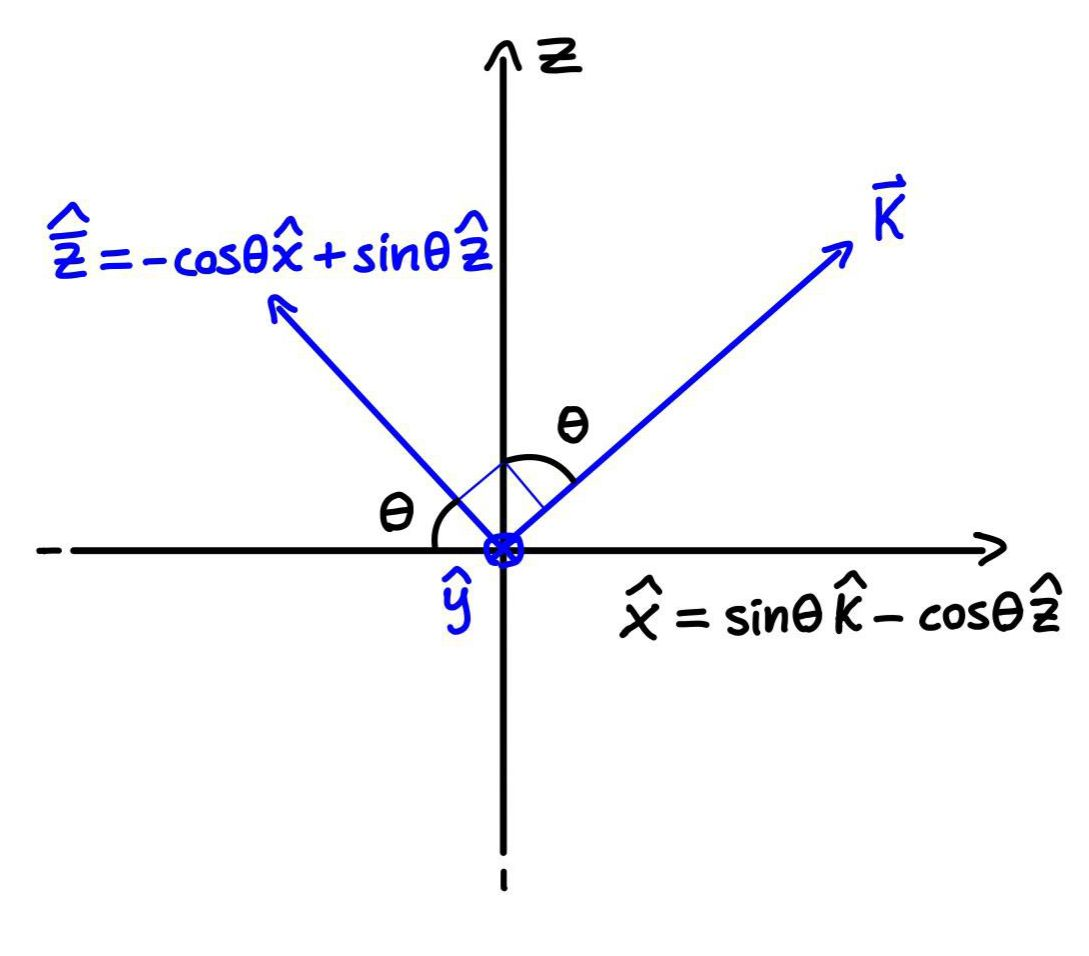
\includegraphics[width=0.6\linewidth]{immagini/riferimento.jpeg}
		\caption{cambio di sistema di riferimento $(\hat x, \hat y, \hat z) \ \ \rightarrow \ \ (\hat k, \hat y, \hat{\bar z})$}
		\label{fig:sist di rif}
	\end{figure}
\end{multicols}

\[  B_0\hat e_z\times (\vec k\times \vec b) \ =\ \begin{vmatrix} 
	\hat x & \hat y & \hat z \\ 
	0 & 0 & B_0\\
	-k_{\parallel} b_y & - k b_{\bar z} & k_{\perp} b_y
\end{vmatrix} \ =\ \hat x\,(k\,B_0\, b_{\bar z})\, -\, \hat y (k_{\parallel}\, b_y\, B_0) + \hat z(0)\]

Ne deriva che la seconda equazione del sitema sia:  

\[\omega \rho_0\vec u = c^2_S \vec k \rho_1 + \frac{1}{4\pi}(kB_0 b_{\bar z} \hat x - k_\parallel b_y B_0 \hat y)\ \ .\] 

Finito questo rimaneggiamento passiamo a fare lo stesso per la terza equazione:

\[ \vec u\,\times\,\vec B_0\ =\ \begin{vmatrix} 
	\hat x & \hat y & \hat{z} \\ 
	u_x & u_y & u_{z}\\
	0 & 0 & B_0
\end{vmatrix} \ =\ B_0 u_y \hat x\, -\,  B_0 u_x \hat{y} \]

\[ \vec k\times (\vec u\times \vec B_0) \ =\ \begin{vmatrix} 
	\hat k & \hat y & \hat{\bar z} \\ 
	k & 0 & 0\\
	-sin\theta B_0 u_y & cos\theta B_0 u_x & cos\theta B_0 u_y
\end{vmatrix} \ =\ -k_\parallel B_0 u_y \hat y + k B_0 u_x \hat z\]

In questo modo abbiamo ridotto il sistema ad uno di :
\[\begin{cases}
	\omega b_y\ =\ -k_\parallel B_0 u_y\\
	\omega \rho_0 u_y\ =\ \frac{B_0}{4\pi}\, k_\parallel b_y
\end{cases}\]

Questo sistema si limite alla direzione y con incognite $u_y$ e $b_y$, mentre il esiste un secondo sitema con $u_z,\, u_x$ e $b_x,\, b_y$, che vedremo nel prossimo paragrafo. 

Otteniamo $\omega u_y = \omega^2 b_y / (k_\parallel B_0)$ e $\rho_0 \omega^2 b_y/(k_\parallel B_0) = B_0 k_\parallel b_y / (4\pi)$ che ci permettono di scrivere una \textbf{relazione di dispersione} per le onde di Alfvén $\forall\ \ \theta$, notando che per $\theta = \pi/2$ non vi sono onde:

\begin{equation}
	\boxed{\ \omega^2\ =\ k^2_\parallel c^2_a\ =\ k^2\, cos^2\theta\, c^2_a\ }
\end{equation}

L'energia si propaga lungo $\hat z$ mentre l'onda si propaga lungo $\hat k$

\[ c_\phi\ =\ \frac{\omega}{k}\ =\ c_a\ cos\theta
\quad \quad \quad \quad \tau_y\ =\ c_a\, \hat z\ =\ \frac{d\omega}{dk}\]


%
%
\vspace{1cm}
\subsection{Onde Magnetosoniche}
Riprendiamo il sistema precedente, questa volta consideriamo la direzione perpendicolare a quella precedente, ignoriamo la direzione y e vediamo cosa succede nel piano $x-k$, stavolta troveremo le \textbf{onde magnetosoniche} che sono \underline{onde comprimibili}:

\[ \begin{cases}
	\omega \rho_1\ =\ \rho_0\ \vec k\cdot \vec u\ =\ \rho_0\ (k_\perp u_x + k_\parallel u_z)\\
	\omega\, \rho_0\, \vec u\ =\ \bar c_s^2 \bar k \rho_1 + \frac{\bar B_0}{4\pi}\hat e_z\times (\vec k\times \vec b)\\
	\omega\,\vec b\ =\ -\vec k\times (\vec u \times \vec B_0)
\end{cases} \]

\[\omega \rho_0 \vec u\ =\ c^2_s\, \frac{\rho_0}{\omega}\, (k_\perp u_x + k_\parallel u_z)\vec k\ +\ \frac{k\, B_0 b_{\bar z}}{4\pi}\, \hat x\ +\ \dots\, \hat y \]

Dalla terza equazione del sistema prendiamo $\omega b_z = k B_0 u_x$, usiamo poi il fatto che $\displaystyle\frac{k^2 B_0^2}{4\pi \rho_0}\, u_x=k^2\, c^2_a u_x$ per ottenere:

\[ \begin{aligned}
	\omega^2 u_x\ &=\ c^2_s\, (k_\perp u_x\, +\, k_\parallel u_z)\, k_\perp\, +\, k^2\,c^2_a\, u_x \\ 
	&=\ \ (k_\perp\, c^2_s\, +\, k^2\, c_a^2)\, u_x\ +\ (c_s^2\, k_\parallel\, k_\perp)\, u_z
\end{aligned} \]

Prendendo $\omega \rho_0 u_z = c^2_s \rho_1 k_\parallel$ scriviamo poi $\omega^2 \rho_0 u_z = c_s^2 k_\parallel \rho_0 (k_\perp u_x + k_\parallel u_z)$ così da giungere al sistema:

\[ \begin{cases}
	(\omega^2\, -\, c^2_s\, k^2_\perp\, -\, k^2\, c^2_a)\, u_x\ -\ k_\parallel\, k_\perp\, c^2_s\, u_z\ =\ 0\\
	k_\parallel\, k_\perp\, c^2_s\, u_x\ -\ (\omega^2\, -\, c_s\, k^2_\parallel)\, u_z\ =\ 0
\end{cases} \]

\[ (\omega^2\, -\, k^2_\perp\, c^2_s\ -\ k^2\, c^2_a)\,(\omega^2\, -\, k^2_\parallel\, c^2_s)\ +\ k^2_\parallel\, k^2_\perp\, c^4_s\ =\ 0 \]

\[ \omega^4 \,-\, \omega^2\, k^2\, (c^2_a\, +\, c^2_s)\, +\, k^2_\parallel\, k^2\, c^2_a\, c^2_s\ =\ 0 \]

\begin{equation}\label{dispersione magnetosoniche}
	\boxed{\ \left( \frac{\omega}{k} \right)^2\ =\ \frac{1}{2}\, \left[\, c^2_a\ +\ c^2_s\ \pm\ \sqrt{(c_a^2\, +\, c_s^2)^2\, -\, 4\, c^2_a\, c^2_s\, cos^2\theta\,}\, \right]\ }
\end{equation}

La scelta del $\pm$ dipende dalla soluzione dell'equazione al quart'ordine, la scelta del segno + definisce in particolare la relazione di dispersione delle onde magnetosoniche \textbf{fast}, mentre la scelta del segno - produce le onde \textbf{slow}.


%
\subsubsection{osserviamo i vari limiti}

Le onde magnetoidrodinamiche fast possono creare shock mentre le onde slow sono soggette a Landau damping.

Osserviamo i vari limiti, partendo dal limite di grandi campi magnetici $\boxed{\beta \ll 1}$ (che si ricollega alla condizione $c_s\ll c_A$), come il caso che si verifica nei tokamak: 

\[\begin{aligned}
	\left( \frac{\omega}{k} \right)^2\ 
	&=\ \frac{1}{2}\, \left[\, c^2_A\ +\ c^2_s\ \pm\ \sqrt{(c_A^2\, +\, c_s^2)^2\, -\, 4\, c^2_A\, c^2_s\, cos^2\theta\,}\, \right]\ =\\
	&\approx\ \frac{1}{2}\, c_A^2\, \left[1\, \pm\, \left(1\,-\, 4\,\frac{c_s^2}{c_A^2}\, cos^2\theta\right)^\frac{1}{2}\,\right]\ \approx\\
	&\approx\  \frac{1}{2}\, c_A^2\,\left[ 1\,\pm\, \left(1\,-\, 2\frac{c_s^2}{c_A^2}\, cos^2\theta\right)\,\right] 
\end{aligned}\]

La scelta del segno + porta ad una magnetosonica simile al modo di Alfvén ma comprimibile, $\boxed{\omega_f\equiv (\omega^+/k)^2=c_A}$.
 
Diversamente la scelta del segno - ci porta a definire $\boxed{\omega_s\equiv (\omega^+/k)^2=c_s \cos\theta}$ in cui compare solamente la velocità del suono.

\vspace{0.5cm}
Osserviamo il limite contrario di campi deboli $\boxed{\beta \gg 1}$ :

\[\begin{aligned}
	\left( \frac{\omega}{k} \right)^2\ 
	&=\ \frac{1}{2}\, \left[\, c^2_A\ +\ c^2_s\ \pm\ \sqrt{(c_A^2\, +\, c_s^2)^2\, -\, 4\, c^2_A\, c^2_s\, cos^2\theta\,}\, \right]\ =\\
	&\approx\ \frac{1}{2}\, c_s^2\, \left[\left(\frac{c_a^2}{c_s^2} + 1\right)\, \pm\, \left[1\,+ 2\,\frac{c_A^2}{c_s^2}\,(1- 2\cos^2\theta)\right]^\frac{1}{2}\,\right]
\end{aligned} \]

In questo caso risulta $\boxed{\omega_f=c_s^2}$ proprio come per le onde acustiche, mentre $\boxed{\omega_s=c_A^2 \cos^2\theta}$ .

Quindi per le onde comprimibili se domina B l'onda veloce è un modo di Alfvén e l'onda slow è una specie di onda sonora.

Se invece non domina B l'onda fast è proprio un'onda sonora e l'onda slow è formalmente un modo di Alfvén.


%
%
%
%
%
\vspace{0.5cm}
\section{Damping di Landau}

Nei capitoli precedenti, abbiamo introdotto la \underline{trattazione statistica a due fluidi}, l'\underline{equazione di Vlasov} e la \underline{MHD}, che descrivono il comportamento dei plasmi su scale macroscopiche e cinetiche. 

Ora ci concentriamo su un fenomeno fondamentale della fisica dei plasmi: l'\underline{interazione onda-particella}, nota come \underline{damping di Landau}.

Questo meccanismo descrive come le onde di plasma possono \underline{perdere energia} (o, in alcuni casi, guadagnarla, cfr. inverse landau damping) a causa dell'interazione con le particelle del plasma, senza che avvenga \underline{termalizzazione} o produzione di calore. È un esempio di \underline{smorzamento non dissipativo}, che si distingue nettamente da fenomeni come la resistività o la viscosità.

\subsubsection{Condizioni per il Damping di Landau}
\begin{itemize}
	\item \emph{Distribuzione delle particelle:}
	Il damping di Landau si verifica quando la funzione di distribuzione delle velocità $f(v)$ delle particelle presenta una \underline{monotonicità locale}. Tipicamente, ci si concentra sul caso in cui $f(v)$ è \underline{monotona decrescente} (se $f(v)$ è monotona crescente, si osserva il fenomeno opposto, noto come \underline{inverso del damping di Landau}, $LD^{-1}$).
	
	\item \emph{Risonanza onda-particella:}
	Il damping avviene quando la \underline{velocità di fase dell'onda} $v_f = \omega/k$ (dove $\omega$ è la frequenza e $k$ il numero d'onda) \underline{coincide} con la velocità di alcune particelle del plasma, cioè $v \sim v_f$. In altre parole, alcune particelle viaggiano \underline{alla stessa velocità dell'onda} e interagiscono con essa in modo risonante.
	\begin{figure}[H]
		\centering
		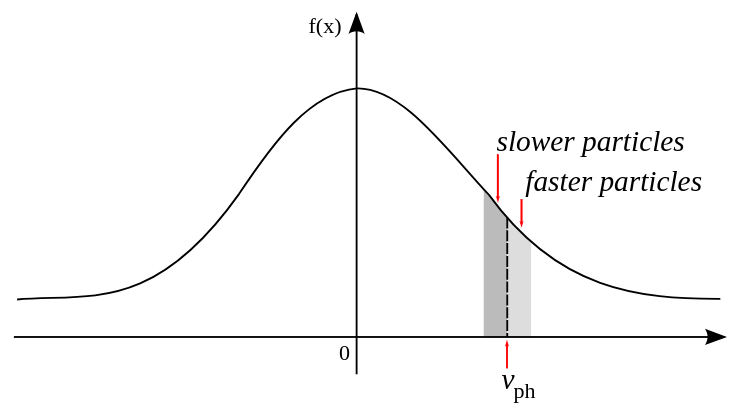
\includegraphics[width=6cm]{immagini/LD.png}
	\end{figure}

	
	\item \emph{Effetto netto:}
	In media, se ci sono \underline{più particelle con $v < v_f$} rispetto a quelle con $v > v_f$, l'onda \underline{perde energia} (damping). Al contrario, se $f(v)$ è monotona crescente, l'onda \underline{guadagna energia} (inverso del damping, $LD^{-1}$).
\end{itemize}

\subsubsection{Plasma Magnetizzato vs. Non Magnetizzato}
\begin{itemize}
	\item \underline{Plasma magnetizzato:}
	In presenza di un campo magnetico, le onde possono propagarsi liberamente lungo la direzione del campo, e il damping di Landau \underline{non avviene}.
	
	\item \underline{Plasma non magnetizzato:}
	In assenza di un campo magnetico, il damping di Landau diventa rilevante. Questo è il caso che tratteremo in dettaglio.
\end{itemize}

Il plasma non è magnetizzato, pertanto: $\boxed{\, \vec{B} = 0\,}$ .

Il campo elettrico medio è nullo e la fluttuazione è esprimibile come gradiente di un potenziale: $\boxed{\,\vec{E} = 0\,}$, $\boxed{\,\vec{E}_1 = -\vec{\nabla}\phi\,}$ .

La funzione di distribuzione per una specie $a$ (elettroni o ioni) è:
\[
f_a(\vec{x}, \vec{v}, t)\ =\ f_{a0}(\vec{v})\, +\, f_{a1}(\vec{x}, \vec{v}, t)\ \ ,
\]

dove $f_{a0}(\vec{v})$ dipende esclusivamente dalla velocità e la distribuzione è pari, ossia $f(v) = f(-v)$, ed è una soluzione all'equilibrio, mentre $f_{a1}(\vec x, \vec v, t)$ è una piccola perturbazione.

Per ciascuna specie vale 


\subsubsection{LD emerge dal framework cinetico: riprendiamo l'eq. di Vlasov.}

\[\frac{\partial}{\partial_t}f_a\ +\ \vec v\cdot \vec\nabla_{\vec x}\, f_a\ +\ \frac{q_a}{m_a}\,\vec E\cdot \vec \nabla_{\vec v}\,f_a\ =\ 0\ \ .\] 

Per descrivere il damping di Landau, è necessario utilizzare l'\underline{equazione di Vlasov}, che governa l'evoluzione della funzione di distribuzione $f(\vec{x}, \vec{v}, t)$ nello spazio delle fasi. L'equazione di Vlasov è particolarmente adatta perché:

\begin{itemize}
	\item \underline{Non richiede una chiusura} (a differenza delle equazioni fluide).
	\item \underline{Conserva l'entropia}: $\dfrac{d}{dt}(f \ln f) = 0$, il che implica che le \underline{isolinee} della funzione di distribuzione possono essere deformate, ma \underline{non possono essere "strappate" o "riconnesse"}.
\end{itemize}

\begin{figure}[H]
	\centering
	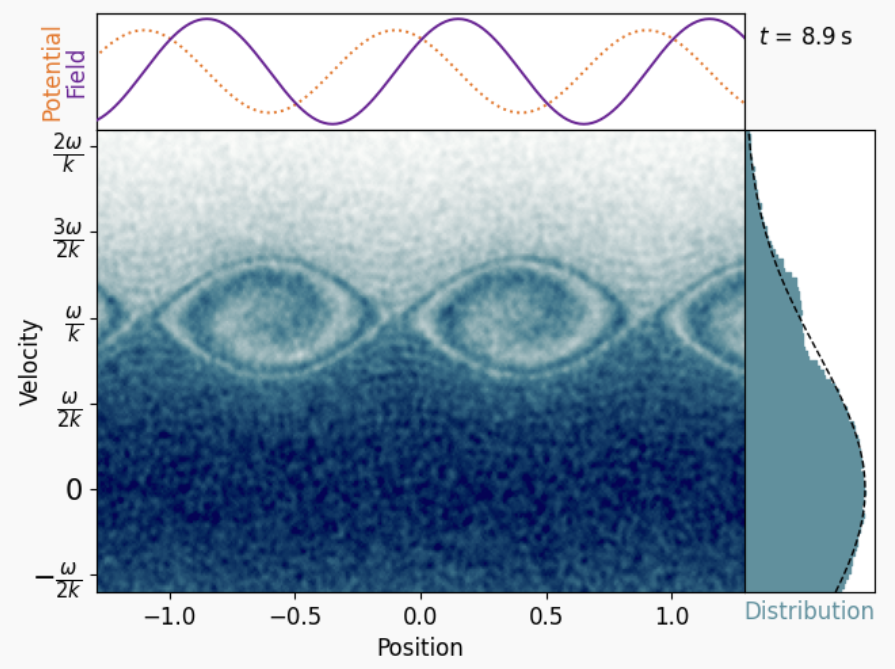
\includegraphics[width=7cm]{immagini/LDvisualized.png}
	\label{Landau Damping}
	\caption{preso da \href{https://kunimune.blog/2023/12/02/an-animated-description-of-landau-damping/}{--> qui.}}
\end{figure}


Le isolinee sono più dense nelle regioni dello spazio delle fasi dove il gradiente di $f$ è maggiore. Se si forma un \underline{vortice} attorno a $v_f$, le isolinee si avvolgono, e si osserva un \underline{cambio di segno della velocità} nel sistema di riferimento dell'onda (fenomeno noto come \underline{trapping}, che discutiamo in seguito).

Quando linearizzo i primi termini: possiamo cancellare l'ordine zero $\frac{\partial f_{a,0}}{\partial t} + \vec v\cdot \vec\nabla_{\vec x} f_{a,0}$ per l'eq. di continuità.

Per quanto riguarda il termine $\vec E\cdot \vec \nabla_{\vec v}f_a$, che linearizziamo in $\frac{q_a}{m_a} (\vec E_0 + \vec E_1)\vec \nabla_{\vec v} (f_{s,0}+f_{s,1})$, le cose sono più delicate:
è vero che all'istante iniziale $\displaystyle\frac{\partial f_{a0}}{\partial v}\gg\frac{\partial f_{a1}}{\partial v}$ ma i gradienti $\partial_v$ evolvono nel tempo e può arrivare un momento in cui la nostra linearizzazione non vale più e in gradienti evolvono in maniera da avere 
$\displaystyle\frac{\partial f_{a0}}{\partial v}\simeq\frac{\partial f_{a1}}{\partial v}$ .

Questo può avvenire dopo un certo \underline{tempo di intrappolamento} $\tau_t$.

In ogni caso, quando vale la linearizzazione ponendo $\vec E_0=0$, abbiamo al primo ordine:

\[\boxed{\ \frac{\partial}{\partial t}\,f_{a1}\ +\ \vec v\cdot \vec\nabla_{\vec x}\, f_{a1}\ +\ \frac{q_a}{m_a}\, \vec E_1\cdot \vec \nabla_{\vec v}\,f_{a0}\ =\ 0}\] 

Useremo anche l'equazione di Poisson:
\[\boxed{\ \vec \nabla\cdot\vec E\ =\ 4\pi\, e\,(n_I-n_e)}\] 
Questa equazione è già linearizzata perchè $\vec E=\vec E_1$ e $n_{0e}=n_{0I}$.
\[-\nabla^2\phi=4\pi e(n_I-n_e)\]

\subsubsection{Caratteristiche Fondamentali del Damping di Landau}
Il damping di Landau è spesso chiamato "smorzamento", ma non è un fenomeno dissipativo. Ecco le sue proprietà chiave:
\begin{itemize}
	\item \textit{Smorzamento $\neq$ dissipazione};
	\item \textit{NON è l'equivalente di un attrito, di una resistività, di una viscosità};
	\item \textit{NON viene prodotto calore o NON aumenta l'entropia};
	\item \underline{È un trasferimento di energia} dall'onda alle particelle (o viceversa), è un fenomeno di interazione \underline{particella-onda};
	\item \underline{L'energia può essere recuperata}: anche se non al 100\%, il trasferimento è potenzialmente reversibile.
\end{itemize}


%
%
%
\subsection{Equazioni di partenza}

Facciamo la trasformata di Fourier per studiare i modi normali dell'onda di plasma e trovare quello meno smorzato, cioè caratterizzato da un coefficiente di smorzamento \(\omega_i\) molto piccolo rispetto alla frequenza reale \(\omega_r\).
Cerchiamo i termini che vanno come $\sim e^{i(\vec k \cdot \vec x - \omega t)}$, dove  \(\boxed{\omega = \omega_r + i\omega_i}\)  è in generale un numero complesso: la parte reale \(\omega_r\) rappresenta l'oscillazione, mentre la parte immaginaria \(\omega_i\) rappresenta lo smorzamento (se \(\omega_i < 0\)) o l'amplificazione (se \(\omega_i > 0\)).

L'equazione di Vlasov linearizzata, in trasformata di Fourier, è:
\[
-\,i\omega\, f_{a,1}\, +\, i\,(\vec{k} \cdot \vec{v})\, f_{a,1}\, +\, \frac{q_a}{m_a}\, (\vec{E} \cdot \nabla_v)\, f_{a,0}\ =\ 0\ \ .
\]
Da questa si trova la soluzione per \(f_1\) ($\vec \nabla \phi_1 \rightarrow i\vec k \phi_1$):
\[
f_{1}(\vec x,\, \vec v,\, t)\ =\ -\,\sum_a\, \frac{q_a}{m_a}\, \frac{(\vec{k} \cdot \nabla_v)\, f_{a,\, 0}}{(\omega\, -\, \vec{k} \cdot \vec{v})}\ \phi_1\ \ \ .
\]

\emph{Nota:} La condizione \(\vec{k} \parallel \vec{E}\) non è esplicitamente derivata qui, ma è implicita nel fatto che per onde longitudinali (come le onde di plasma), il campo elettrico è parallelo a \(\vec{k}\) (perché \(\vec{E}_1 = -\nabla \phi_1\) e \(\phi \sim e^{i\vec{k} \cdot \vec{x}}\)).

L'equazione di Poisson ($ikE_1=4\pi e (n_i - n_e)$) linearizzata è:
\[
-(ik)^2\, \phi_1\ =\ 4\pi e \int (f_{i,1} - f_{e,1})\, d\vec{v}.
\]
La soluzione del sistema di equazioni è:

\begin{equation}
	\label{LD soluzione}
	k^2\, \phi_1\ =\ -4\pi e\, \sum_a \frac{q_a}{m_a} \int \frac{(\vec{k} \cdot \nabla_v) f_{0a}}{(\omega - \vec{k} \cdot \vec{v})}\, d\vec{v} \
	\phi_1\ \ ,
\end{equation}

da cui si ottiene la \textbf{relazione di dispersione}:

\begin{equation}
	\label{LD dispersion 1}
	\boxed{\, k^2\ =\ -4\pi e\, \sum_a \frac{q_a}{m_a}\, \int \frac{(\vec{k} \cdot \nabla_v) f_{0a}}{(\omega - \vec{k} \cdot \vec{v})}\, d\vec{v}\ \ .}
\end{equation}



%

\subsubsection{Onda di plasma a ioni fissi}

Consideriamo un'onda di plasma con frequenza tale che gli ioni non facciano in tempo a reagire. Il contributo degli ioni si limita quindi a mantenere la quasi-neutralità tramite \(n_0\). Se non facessimo questa assunzione, troveremmo anche soluzioni con onde ion-acoustic (IA).

Se l'onda di plasma si propaga in direzione \(x\), possiamo integrare la distribuzione in \(dv_y\) e \(dv_z\), perché il termine \(\vec{k} \cdot \nabla_v\) non coinvolge quelle direzioni. L'integrale diventa quindi un integrale 1D, dato che l'onda si propaga in un'unica direzione:
\[
\vec{k} \cdot \nabla_v\, \to\, k\, \partial_u\ \ , \qquad u \equiv v_x\ \ .
\]

È conveniente definire la funzione di distribuzione normalizzata a 1 in termini di \(n_0\), perché si riconosce che, a meno di \(n_0\), la frequenza di plasma degli elettroni \(\omega_e\) moltiplica l'integrale:
\[
g(u)\, =\, \frac{f(u)}{n_0}\ ; \qquad \int f(u) du\, =\, n_0\ \to\ \int g(u) du\, =\, 1\ \ .
\]

Si ottiene quindi, partendo da eq.\ref{LD soluzione} :

\[
\phi_k\ =\ -\frac{\omega_e^2}{k^2}\, \int \frac{(\vec{k} \cdot \nabla_v)\, f_{0e}}{(\omega - \vec{k} \cdot \vec{v})}\, d\vec{v} \, \phi_k\ \ \ ,
\]

che porta eq.\ref{LD dispersion 1} alla relazione di dispersione:

\begin{equation}
	\label{LD dispersion 2}
	\boxed{\,1 \ +\ \frac{\omega_e^2}{k^2}\, \int\, \frac{\partial_u\, g(u)}{\left(\frac{\omega}{k}\, -\, u\right)} du\ =\ 0}\ \ \ .
\end{equation}




%
%
%
\subsection{intrappolamento e non linearità} 

L'intrappolamento delle particelle avviene quando un'onda di plasma con velocità di fase \(v_f \sim \omega_p/k\) interagisce con particelle che si muovono a velocità \(v \sim v_f\). Nel sistema di riferimento dell'onda (SDR), queste particelle vedono un campo elettrostatico statico ($E=\hat E\sin(kx-\omega_pt)$) e vengono intrappolate in una buca di potenziale, oscillando con moto armonico ($m\ddot x=-e\hat E\sin kx \simeq -e\hat Ekx$).

Il comportamento del sistema è governato da tre tempi:
\begin{itemize}
	\item \(\tau_t = \sqrt{\dfrac{m}{e\hat{E}k}}\): tempo di intrappolamento, dipendente dall'ampiezza dell'onda;
	\item \(\tau_L= \displaystyle\frac{1}{k^3\lambda_D^3}e^{-(\frac{3}{2}+\frac{1}{2k^2\lambda_D^2})}\): tempo caratteristico del damping di Landau;
	\item \(\tau_D \sim \omega_p^{-1}\): tempo caratteristico dinamico del plasma.
\end{itemize}
L'intrappolamento è rilevante solo se \(\tau_D < \tau_t < \tau_L\). Se \(\tau_t > \tau_L\), l'onda viene smorzata prima che l'intrappolamento possa avere effetto.
	
Le particelle intrappolate modificano la distribuzione in velocità, appiattendola attorno a \(v_f\). Il numero di particelle intrappolate aumenta nel tempo, e alcune possono invertire la direzione della velocità nel SDR. Questo fenomeno è non dissipativo: l'energia non viene convertita in calore, ma trasferita tra onda e particelle.
	
L'evoluzione della distribuzione perturbata \(f_1\) è descritta dall'equazione di Vlasov linearizzata:
\[
\frac{\partial f_1}{\partial t}\, +\, v \frac{\partial f_1}{\partial x}\ =\ \frac{e\hat{E}}{m}\, \sin(kx - \omega t)\, \frac{\partial f_0}{\partial v}\ \ .
\]

Sviluppando attorno a \(v \sim v_f\), si osserva che \(\partial_v f_1\) cresce quadraticamente nel tempo, invalidando l'ipotesi di linearità in un tempo \(\tau_t\).

\[f_1\ =\ f_1(v,t=0)\,\cos(kx-kvt)\ -\ \frac{e\hat E}m\frac{\partial f_0}{\partial v}\bigg[ \frac{\cos(kx-\omega _e t)}{kv-\omega_e}\, -\, \frac{\cos(kx-kv t)}{kv-\omega_e}\bigg]\] 

\[
\partial_v f_1\ \approx\ \frac{ek\hat{E}}{m}\, t^2\, \partial_v f_0\, \frac{\cos(kx - \omega t)}{2}\ \propto\ t^2\ \ .
\]
Questo mostra che, in un tempo \(\tau_t \sim \sqrt{\dfrac{m}{e\hat{E}k}}\), la derivata \(\partial_v f_1\) diventa dell'ordine di 1, invalidando l'ipotesi di linearità. L'intrappolamento, quindi, modifica la funzione di distribuzione e segna il limite fisico della linearizzazione.
 



%
%

\vspace{0.5cm}
\begin{approfondimento}{Ripasso di metodi matematici}
	
	\begin{itemize}
		\item Una funzione $f(z)=u(x,y)+iv(x,y)$ è olomorfa in $D\in \mathbb C$ se è differenziabile e la sua derivata prima è continua;
		\item Se integriamo $\oint_{C^+_R} \frac{1}{z-z_0}$ sulla circonferenza in senso antiorario attorno al punto $z_0$, $C^+_R={z(\theta)=z_0 + Re^{i\theta},\ \theta\in [0,2\pi)}$, troveremmo che $\int_0^{2\pi} \frac{1}{z-z_0} \frac{dz}{d\theta}d\theta = \int_0^{2\pi} \frac{1}{Re^{i\theta}}(iRe^{i\theta})d\theta= 2\pi\, i$;
		\item Per il \underline{teorema di Cauchy} presa $f(z)$ funzione analitica in un dominio D semplicemente connesso, allora $\oint_\Gamma f(z) dz = 0$ per ogni contorno chiuso $\Gamma$ completamente contenuto in D;
		\item Dal secondo teorema di Cauchy si trova che $\oint_\Gamma \frac{f(z)}{z-z_0}=2\pi i f(z_0)$ fissato un punto interno arbitrario $z_0\in D$;
		\item un punto singolare si dice "eliminabile" se esiste il limite della funzione per la variabile che tende a quel punto, si dice "polo di ordine m" se lo sviluppo di Taylor-Laurent è $f(z)=\frac{c_{-m}}{(z-z_0)^m} +\dots + \frac{c_0}{(z-z_0)} + \sum_{n=0}^\infty c_n (z-z_0)^n$ ed esiste quindi $\lim_{z\to z_0}f(z)(z-z_0)^m = c_{-m}$, si dice invece che il punto singolare è "essenziale" se questi limiti non esistono;
		\item Una funzione analitica f(z) nell'intorno di un punto singolare isolato $z_0$ può essere sviluppata in serie di Taylor-Laurent: $f(z)=\sum_{n=-\infty}^{+\infty} \frac{1}{2\pi i} \oint_C \frac{f(\eta)}{(\eta - z_0)^{n+1}}d\eta (z-z_0)^n$;
		\item $\text{Res}[f(z), z_0] = \frac{1}{2\pi i} \oint_C f(\eta)d\eta$, se $z_0$ è un punto singolare eliminabile $\text{Res}[f(z), z_0] = 0$, se $z_0$ è un polo di ordine 1 $\text{Res}[f(z), z_0] = \lim_{z \to z_0}(z-z_0)f(z)$, se $z_0$ è un polo di ordine m invece $\text{Res}[f(z), z_0] = \frac{1}{(m-1)!} \lim_{z \to z_0}\frac{d^{m-1}}{dz^{m-1}}[(z-z_0)^m f(z)]$  ;
		\item Per il teorema interno dei residui se la nostra funzione è analitica all'interno di un contorno chiuso, con un numero finito di punti singolari, è possibile sostituire l'integrale su tale contorno con una somma dei residui 
		\[\oint_\Gamma f(z)\, dz\ =\ 2\pi\, i\, \sum_{k=1}^{N}\,\text{Res}[f(z),\, z_k]\] 
		\item La parte principale secondo Cauchy si calcola come $\text{P}\left(\int_a^b f(z) dz = \right)=\lim_{\epsilon \to 0}\left(\int_a^{x_0-\epsilon} f(z) dz +\int _{x_0+\epsilon}^b f(z) dz\right)$ con $x_0$ singolarità;
		\item Quando vogliamo eliminare un punto singolare sull'asse reale dobbiamo aggirarlo con un semicerchio, fare quindi la parte principale sull'asse reale per non prendere il punto di singolarità $\omega_0$, si somma il semicerchio che contribuisce per $-i\pi\text{Res}[f,\omega_0]$ e poi si chiude la curva con il semicerchio in senso antiorario che si annulla se è rispettato il lemma di Jordan ($|f(z)|<M/|z|$ per $z\to \infty$). 
	\end{itemize}
	
\end{approfondimento}


%
%
%
\subsection{Regime di propagazione senza damping} 

Prendiamo un'onda con $v_f\gg v_{th}$, in questo caso la velocità di fase non si sovrappone alla distribuzione e possiamo dire che non ci sono elettroni che si muovono localmente con velocità $u\sim v_{th}$, questo significa che la derivata della distribuzione è a maggior ragione nulla. 


Matematicamente questo significa che in corrispondenza della singolarità, 

\[\dfrac{\omega}{k}\,-\,u\ =\ 0\ \ ,\] 

che porterebbe ad una divergenza. Rimane da risolvere l'integrale:

\[\int\, \frac{\partial_u\, g(u)}{(\frac{\omega}{k}-u)}\, du\]  

integro per parti e quando devo valutare il prodotto  tra le primitive ai bordi del dominio posso mettere tutto a zero (non ho particelle con velocità infinita!). 

\[\int\frac{\partial_u\,g(u)}{(\frac{\omega}{k}-u)}\,du\ \, =\, \ \cancelto{0}{\frac{g(u)}{(\frac{\omega}{k}-u)^2}\bigg|_{-\infty}^{+\infty}}\ -\ \int \frac{g(u)}{(\frac{\omega}{k}-u)^2}du \]

Ci dobbiamo occupare del secondo termine, la distribuzione conta qualcosa nella zona  $\boxed{ u \ll \omega / k }$ , questo equivale a dire che possiamo espandere il denominatore attorno a $u=0$:

\[\frac{1}{(\frac{\omega}{k}-u)^2}\ \simeq\ 
 \frac{1}{(\frac{\omega}{k})^2}\ +\ \frac{2u}{(\frac{\omega}{k})^3}\ +\ \frac{3u^2}{(\frac{\omega}{k})^4}\ +\ ...\]

Ora uso il fatto che la distribuzione è pari per cancellare il termine dispari nell'integrale 

\[1\ -\ \frac{\omega_e^2}{k^2} \int \frac{\partial_ug(u)}{(\frac{\omega}{k}-u)}\,du\ \ =\ \ 1\ -\  \int_{-\infty}^{+\infty} g(u)\, \frac{\omega_e^2}{k^2} \, \bigg[\frac{k^2}{\omega^2}\,+\,\cancel{\frac{2uk^3}{\omega^3}}\,+\,\frac{3u^2k^4}{\omega^4}\bigg]\, du \]  

Uso il fatto che la sitribuzione è normalizzata ad 1 ($\int g(u)du=1$) e anche che valgono $\int g(u)\, u\,d\vec v=0$ e $\int g(u)\, u\,d\vec v=v^2_{th}$.

\[\int\, g(u)\,du\,=\,1\ \ ,\qquad \int g(u)\,u^2\,du\ =\ v_{th}^2\] 

Dopo eq.\ref{LD dispersion 1}, \ref{LD dispersion 2} , troviamo la relazione di dispersione: 

\[\boxed{\,1\ -\ \frac{\omega_e^2}{\omega^2}\ -\ \frac{3k^2v^2_{th}\omega_e^2}{\omega^4}\ =\ 0}\ \ .\]

Ricordiamoci sempre che  $\dfrac{v_{th}^2 k^2}{\omega_e^2}\ll1\iff v_f\gg v_{th}$ , per cui:

\[\omega^2\ =\ \frac{\omega_e^2\,\pm\, \sqrt{\omega_e^4\bigg[1+\dfrac{12k^2v_{th}^2}{\omega_e^2}\bigg]}}{2}\ \simeq\ \frac{\omega^2_e\, \pm\, \omega_e^2\bigg[1+\dfrac{6k^2v_{th}^2}{\omega_e^2}\bigg]}{2}\]

Questa equazione ha due soluzioni ma solamente una è fisica (quella con il segno +).
 
Questo risultato è molto importante perché analogo nel caso con damping:
\[\boxed{\ \omega_+^2\ =\ \omega_e^2\, +\, 3 k^2 v_{th}^2\ }\ \ ,\]

è il caso di confrontare questo risultato con la relazione di dispersione ottenuta con le equazioni fluide chiuse con una politropica 
\[\omega^2=\omega_e+\gamma k^2 v_{th}^2\]
Ci sono alcune cose che è bene notare \begin{enumerate}
	\item L'idea di utilizzare una chiusura politropica non è poi così folle. 
	\item molti dicono che questo $\gamma=3$ era previsto perché è il coefficiente tipico per un gas monoatomico... Califano invece dice che è soltanto una coincidenza senza un particolare significato profondo.
	\item  alla maggior parte degli stimoli, I plasmi reagiscono in prima approssimazione alla frequenza di plasma indipendentemente da $k$. 
\end{enumerate} 



%
%
%
\subsection{Regime di propagazione con damping}  

Ripartiamo dalla nostra relazione del dielettrico, se $\epsilon(k,\omega)=0$ allora abbiamo un modo normale, in generale abbiamo

\[\boxed{\ \epsilon(k,\omega)\ =\ 1\,-\,\frac{\omega_e^2}{k^2}\int\frac{\partial_ug(u)}{(u-\dfrac{\omega}{k})}du\ }\] 

Ricordiamoci sempre che stiamo facendo la trasformata di Fourier cercando il modo che sopravvive più a lungo che corrisponde ad un \textit{polo lontano} con $|\omega_i|\ll|\omega_r|$, praticamente stiamo dicendo che il damping c'è ma poco. 

Per contestualizzare bene quello che stavamo facendo prima il polo c'era lo stesso ma era in una zona dove il damping non avviene per come è popolata la distribuzione. 

Sviluppiamo il nostro dielettrico attorno a $\omega_r$, proprio considerando $|\omega_i|\ll|\omega_r|$: 

\[\epsilon(k,\omega)\ \simeq\ \epsilon_r(k,\omega_r)\, +\, i\epsilon_i(k,\omega_r)\, +\, i\omega_i\frac{\partial \epsilon_r}{\partial\omega}\bigg|_{\omega=\omega_r}\, -\, \cancelto{\text{ordine successivo}}{\omega_i\frac{\partial \epsilon_i}{\partial\omega}\bigg|_{\omega=\omega_r}}\ \overset{!}{=}\ 0\ \ .\] 

Si impone che siano nulle sia la parte reale che la parte immaginaria (per trovare il modo normale). 

Dalla parte immaginaria ottengo 

\[\epsilon_i=-\omega_i\frac{\partial\epsilon_r}{\partial \omega}\bigg|_{\omega_r}\implies \epsilon_i\sim\omega_i\] 
Dalla parte reale emerge che il termine di derivata va come $\sim \omega_i^2$ e di conseguenza lo posso trascurare, cos' come $\epsilon_r$. In generale la parte reale è zero, a meno di correzioni del second'ordine, che non ci interessano. 
\[\omega_i=\dfrac{-\epsilon_i}{\dfrac{\partial \epsilon_r}{\partial \omega}}\] 

Abbiamo un polo molto vicino all'asse dei reali e noi ci giriamo attorno, poi facciamo il giro circolare con $|\omega|\to\infty$ che fa zero.

Bisogna utilizzare la formula di PLEMELJ

\[\lim_{\epsilon\to0}\,\frac{1}{x\pm i\epsilon}\ =\ \mathcal P\,\frac{1}{x}\ \mp\ i\pi\,\delta(x)\]
 
\[\frac{1}{u-a}\ =\ \mathcal{P}\,\bigg(\frac{1}{u-a}\bigg)\,+\,i\pi\,\delta(u-a)\] 

\[\mathcal{P}\,\bigg(\frac{1}{u-a}\bigg)\ \equiv\  \lim_{\epsilon\to 0}\, \bigg[\,\int_{-\infty}^{a-\epsilon}\frac{f(u)}{u-a}du\, +\, \int^{\infty}_{a+\epsilon}\frac{f(u)}{u-a}du\,\bigg]\]

Questo integrale ha la proprietà che le due divergenze  sono uguali ma opposte e quindi si annullano a vicenda. Come se non avessi elettroni nel polo.

Questo mi permette di andare avanti nel calcolo come nel caso precedente assumendo che $v_f^2\gg v_{th}^2$ e trovare un risultato completamente analogo 

\[\epsilon_r\ =\ 1\, -\, \frac{\omega_e^2}{\omega^2}\, -\, \frac{3k^2v_{th}^2\omega_e^2}{\omega^4}\]

Questo è un caso un pochino borderline perché non siamo nelle condizioni più favorevoli per avere il damping e la risonanza avviene con "pochi" elettroni. 

Purtroppo il calcolo dell'integrale in maniera analitica al di fuori di questa assunzione è molto complicato, e non solo... in un regime di forte smorzamento di landau ($\omega/k\sim v_{th}$) non vale la linearizzazione assunta inizialmente e quindi bisogna procedere con l'integrazione numerica di Vlasov porta a risultati sorprendentemente coerenti (nell'ordine del percento)

Ora se faccio la derivata (calcolata in $\omega=\omega_r$) trovo due termini, uno dei quali è trascurabile in quanto $v_f^2\gg v_{th}^2$. 

\[\frac{\partial \epsilon_r}{\partial\omega}\bigg|_{\omega=\omega_r}\ =\ -2\,\frac{\omega_e^2}{\omega_r^3}\, -\, \cancelto{0}{\frac{12k^2v_{th}^2\omega_e^2}{\omega_r^5}}\]  

e a questo punto posso ricucire insieme tutti quanti i pezzi e trovare la parte immaginaria della frequenza, che poi sarebbe il \underline{coefficiente di smorzamento}. 

Bisogna gestire correttamente la $\delta$ che mi fa calcolare la funzione di distribuzione in $u=\omega_r/k$. 

\[\boxed{\ \omega_i\ =\ \dfrac{-\epsilon_i}{\partial _\omega\epsilon_r}\ =\ \frac{\pi\,\omega_e^3}{2\,k^2}\,\partial_ug(u)\bigg|_{u=\omega_r/k}\ }\]  



%
%
%
\subsection{Soluzione con distribuzione generica}
\[\boxed{\omega_i=\dfrac{-\epsilon_i}{\partial _\omega\epsilon_r}=\frac{\pi\omega_e^3}{2k^2}\partial_ug(u)\bigg|_{u=\omega_r/k}}\]   
Questa è la parte immaginaria della frequenza ottenuta con la FT, se teniamo presente che stavamo cercando una soluzione con $e^{-i(\omega_r+i\omega_i) t}$ si vede che la parte immaginaria costtistuisce uno smorzamento (o un'amplificazione) esponenziale $\sim e^{\omega_it}$.\\In particolare ci piace molto il fatto che $\omega_i\propto \partial_ug(u)$ sicché quando $g(u)$ è decrescente si ha lo smorzamento, quando $g(u)$ cresce si ha LD$^{-1}$ mentre non succede niente di niente se la distribuzione è piatta. Questo intuitivamente ci piace anche se pensiamo al fenomeno dell'intrappolamento anche se cade l'ipotesi della linearizzazione.  

%
%
%
\subsection{Soluzione con maxwelliana} 
\textit{"Non ho bisogno di una maxwelliana per avere Damping, ma ho bisogno di una maxwelliana per fare il conto"}  scansoequivoci la maxweliana è siffatta:
\[f=\frac{n_0}{\sqrt{(2\pi)^3}v_{th}^3}e^{-\dfrac{v_x^2+v_y^2+v_z^2}{2v_{th}^2}}\]
La nostra funzione di distribuzione in particolare è normalizzata e 1D
\[g(u)=\frac{1}{\sqrt{2\pi}v_{th}}e^{-\dfrac{u^2}{2v_{th}^2}}\]
Da cui si trova agevolmente la parte immaginaria della frequenza che corrisponde al damping. 
\[\boxed{\omega_i=-\omega_e\sqrt{\frac{\pi}{8}}\frac{1}{(k\lambda_D)^3}e^{-\dfrac{3+k^2\lambda_D^2}{2}}}\]
Si vede che come atteso lo smorzamento scompare completamente per $k^2\lambda_D\to0$. 

